%!TEX root = ./template-skripsi.tex
%-------------------------------------------------------------------------------
%                            BAB III
%               			PEMBAHASAN
%-------------------------------------------------------------------------------

\chapter{IMPLEMENTASI PROGRAM}

Secara umum tahapan pengembangan sistem dalam metode \emph{System Development Life Cycle} (SDLC) adalah analisis kebutuhan perangkat lunak, desain sistem, konstruksi atau pengembangan, dan pengujian atau evaluasi.


\section{Analisis Kebutuhan}

Kebutuhan mengenai sistem didapat berdasarkan hasil analisis perbandingan sistem \textit{tracer study} yang sudah ada yaitu, Sistem \textit{Tracer Study} Dikti, dan Sistem Informasi \textit{Tracer Study} Universitas Negeri Jakarta [Lampiran A]. Selain itu, melalui pengumpulan data yang diperoleh dari analisis kebutuhan prodi Ilmu Komputer [Lampiran C]. Berikut beberapa kebutuhan yang didapat:
\begin{enumerate}
	\item Memiliki lima pengguna, yaitu admin, koorprodi, alumni, dan pengunjung yang memiliki sub-aktor pengguna alumni. 
	\item Admin dapat mengelola data alumni dan pengguna alumni, membuat kuesioner, menyunting konten beranda, dan menampilkan hasil \textit{tracer study}
	\item Koorprodi dapat menampilkan data alumni dan pengguna alumni, dan dapat menampilkan hasil \textit{tracer study}
	\item Alumni dapat mengelola data diri, riwayat pekerjaan dan mengisi kuesioner yang telah dibuat oleh admin
	\item Pengunjung dapat melakukan pencarian alumni, melihat daftar pengguna alumni, dan melihat data hasil \textit{tracer}. 
	\item Pengguna alumni dapat mengisi form kuesioner.
\end{enumerate}

\section{Desain Sistem}

Pada tahap ini perancangan dan pemodelan sistem dituangkan dalam bentuk visual mulai dari \textit{Use Case Diagram, Activity Diagram, Class Diagram, Entity Relationship Diagram} dan \textit{mock-up} atau rancangan dari tampilan sistem. 

\subsection{\emph{Use Case Diagram}}
\textit{Use Case} digunakan untuk mengetahui fungsi apa saja yang terdapat di dalam suatu sistem dan siapa saja yang berhak menggunakan fungsi-fungsi tersebut. Pada sistem ini terdapat lima aktor yaitu admin, koorprodi, alumni, dan penunjung yang memiliki sub-aktor pengguna alumni. Peran-peran aktor tersebut adalah sebagai berikut:
\begin{enumerate}
	\item Admin
	\begin{itemize}
		\item Admin dapat mengelola data alumni
		\item Admin dapat mengelola data pengguna alumni
		\item Admin dapat membuat form kuesioner \textit{tracer study}
		\item Admin dapat menyunting kata pengantar \textit{tracer study} pada beranda alumni 
		\item Admin dapat melihat hasil \textit{tracer study} 
	\end{itemize}
	\item Koorprodi 
	\begin{itemize}
		\item Koorprodi dapat melihat data alumni
		\item Koorprodi dapat melihat data pengguna alumni
		\item Koorprodi dapat melihat hasil \textit{tracer study}
	\end{itemize}
	\item Alumni
	\begin{itemize}
		\item Alumni dapat mengelola data diri dan riwayat pekerjaan
		\item Alumni dapat mengisi form kuesioner \textit{tracer study}
		\item Alumni dapat melihat daftar pengguna alumni beserta alumni yang bekerja
	\end{itemize}
	\item Pengunjung
	\begin{itemize}
		\item Pengunjung dapat melihat daftar alumni
		\item Pengunjung dapat melihat daftar pengguna alumni
		\item Pengunjung dapat melihat data \textit{tracer}
	\end{itemize}
	\item Pengguna Alumni
	\begin{itemize}
		\item Pengguna Alumni dapat mengisi form kuesioner
	\end{itemize}
\end{enumerate}

Berikut adalah \textit{Use Case Diagram} dari Sistem Informasi \textit{Tracer Study} Ilmu Komputer FMIPA UNJ

\begin{figure}[H]
	\centering
	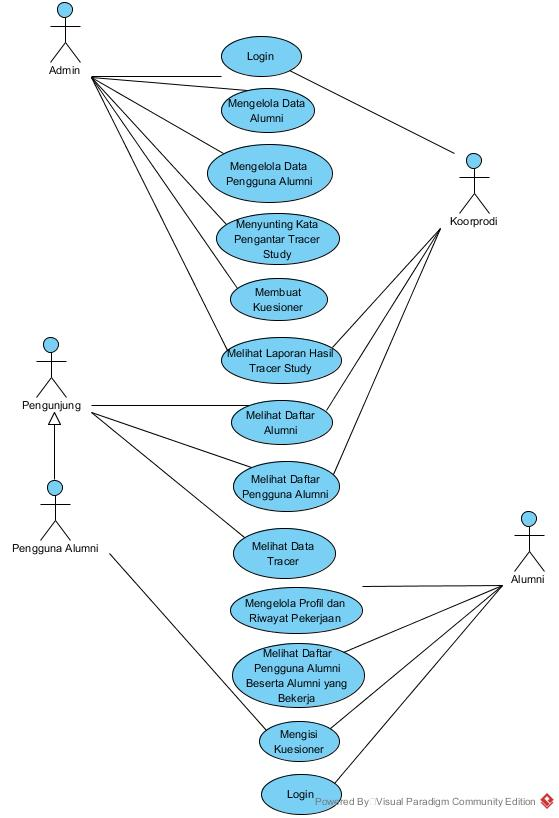
\includegraphics[width=1.0\textwidth]{gambar/usecase}
	\caption{\emph{Use Case Diagram} Sistem Informasi \textit{Tracer Study} Ilmu Komputer}
	\label{usecase_diagram}
\end{figure}


\subsection{\emph{Entity Relationship Diagram}}

ERD dibawah ini menggambarkan masing-masing entitas dan relasi antar entitas untuk basis data Sistem Informasi \textit{Tracer Study} Ilmu Komputer yang akan menyimpan data yang dibutuhkan sistem di antaranya data alumni, pengguna alumni, kuesioner dan hasil kuesioner. Pada ERD ini dibuat tabel pekerjaan dimana berfungsi untuk menampung data riwayat pekerjaan setiap alumni dan tabel instansi untuk menyimpan perusahaan-perusahaan tempat alumni bekerja. Kedua tabel tersebut berelasi dengan tabel alumni dan pengguna alumni. Tabel kuesioner berfungsi untuk menampung kuesioner baik kuesioner alumni maupun pengguna alumni dan berelasi dengan tabel pertanyaan untuk menyimpan pertanyaan-pertanyaan kuesioner. Selain itu disediakan tabel jawaban untuk menampung jawaban kuesioner. Berikut pemodelan ERD sistem informasi \textit{Tracer Study} Ilmu Komputer. 

\begin{figure}[H]
	\centering
	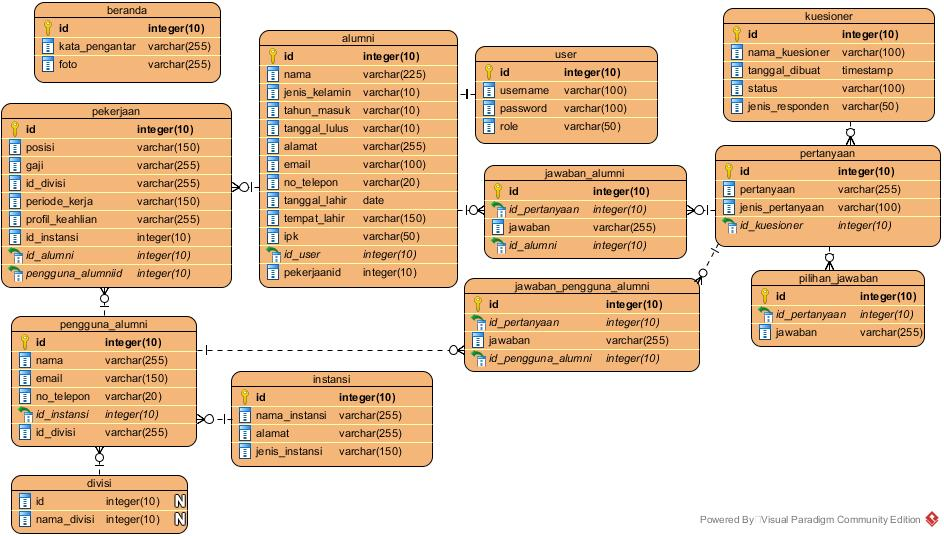
\includegraphics[width=1.0\textwidth]{gambar/erd}
	\caption{\emph{Entity Relationship Diagram} Sistem Informasi \textit{Tracer Study} Ilmu Komputer}
	\label{entityrelationship_diagram}
\end{figure}

\subsection{\textit{Class Diagram}}

Pemodelan \textit{Class Diagram} pada Sistem Informasi \textit{Tracer Study} Ilmu Komputer memiliki sembilan \textit{Class}. Terdapat \textit{Class user} yang menyimpan metode \textit{login, logout,} dan mengganti \textit{password}. \textit{Class} ini memiliki tiga \textit{subclass} dimana dapat mengakses metode dan atribut dari\textit{ Class} tersebut yaitu admin, koorprodi, dan alumni.\textit{ Class} kuesioner untuk menampung kuesioner dan berelasi dengan \textit{Class} pertanyaan yang berisi metode untuk mengelola pertanyaan kuesioner. Selanjutnya terdapat \textit{Class} hasil berfungsi untuk mengelola dan menampilkan hasil kuesioner dan \textit{Class} pekerjaan untuk mengelola data pekerjaan alumni. Berikut adalah \textit{Class Diagram} dari sistem Informasi \textit{Tracer Study} Ilmu Komputer

\begin{figure}[H]
	\centering
	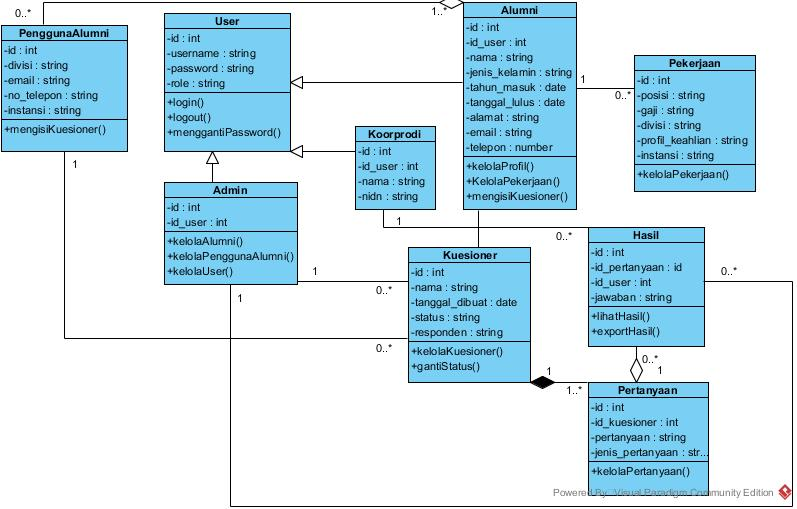
\includegraphics[width=1.0\textwidth]{gambar/class}
	\caption{Desain \emph{Class Diagram} Sistem Informasi \textit{Tracer Study} Ilmu Komputer}
	\label{class_diagram}
\end{figure}


\subsection{\textit{Activity Diagram}}

Desain \textit{Activity Diagram} pada sistem ini dibagi menjadi lima diagram, yaitu membuat form kuesioner untuk admin, melihat hasil atau laporan \textit{tracer study} untuk admin dan koorprodi, mengisi riwayat pekerjaan untuk alumni dan mengisi form kuesioner untuk alumni dan pengguna alumni. Berikut ini \textit{Activity Diagram} dari Sistem Informasi \textit{Tracer Study} Ilmu Komputer

\begin{figure}[H]
	\centering
	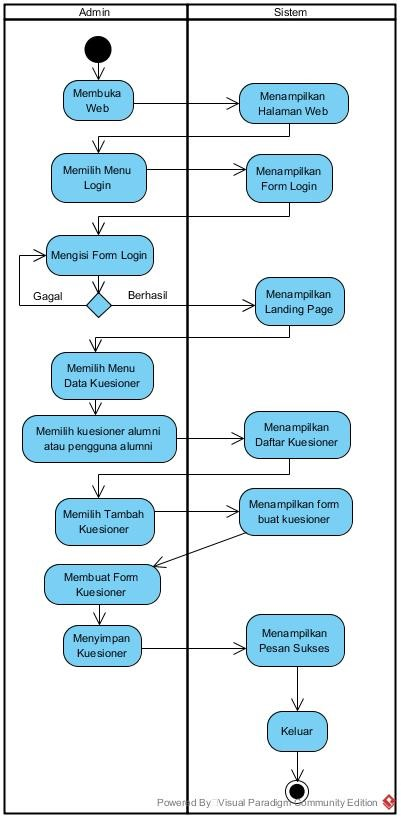
\includegraphics[width=8cm,height=15cm]{gambar/Activitykelolakuesioner}
	\caption{\emph{Activity Diagram} Membuat Kuesioner \textit{Tracer Study}}
	\label{activity_kelolakuesioner}
\end{figure}

Gambar 3.4 menggambarkan aktivitas dalam membuat form kuesioner baik untuk kuesioner alumni maupun pengguna alumni yang dilakukan oleh admin. Dalam pembuatan form kuesioner, admin dapat menambahkan pertanyaan kuesioner dimana disediakan empat jenis pertanyaan, yaitu pertanyaan isian, pilihan, pilihan ganda, dan pertanyaan dengan jawaban skala.  

\begin{figure}[H]
	\centering
	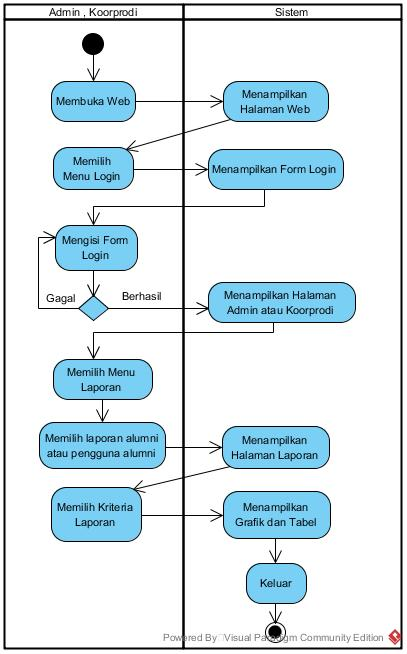
\includegraphics[width=9cm,height=15cm]{gambar/Activitymelihatlaporan}
	\caption{\emph{Activity Diagram} Melihat Laporan \textit{Tracer Study}}
	\label{activity_melihatlaporan}
\end{figure}

Pada \textit{Activity Diagram} melihat laporan, admin dan koorprodi dapat melihat laporan hasil \textit{tracer study} baik alumni dan pengguna alumni. Sebelum menampilkan laporan, admin dan koorprodi mengisi kriteria yang dipilih yaitu berdasarkan jenis kuesioner, pertanyaan yang ingin dilihat hasilnya, dan juga tahun lulus, kemudian sistem akan menampilkan hasil \textit{tracer study} dalam bentuk grafik dan tabel. Selain itu, pada halaman hasil \textit{tracer study} admin dan koorprodi dapat mengekspor data \textit{tracer} dalam format \textit{excel}. 
%kemungkinan halaman laporan berubah

\begin{figure}[H]
	\centering
	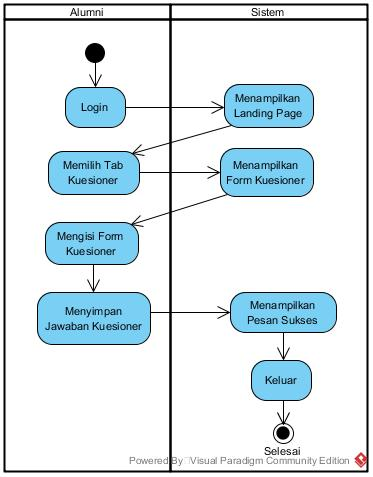
\includegraphics[width=10cm,height=12cm]{gambar/Activitykuesioneralumni}
	\caption{\emph{Activity Diagram} Mengisi Kuesioner Alumni}
	\label{activity_kuesioneralumni}
\end{figure}

Gambar 3.6 menjelaskan aktivitas mengisi kuesioner yang dilakukan oleh alumni. Pada sistem ini juga disediakan form riwayat pekerjaan agar terlihat rekam jejak dari setiap pekerjaan alumni yang pernah digeluti dan juga untuk mengisi data mengenai pengguna alumni. Desain tampilan dari aktivitas mengisi riwayat pekerjaan untuk alumni sebagai berikut.

\begin{figure}[H]
	\centering
	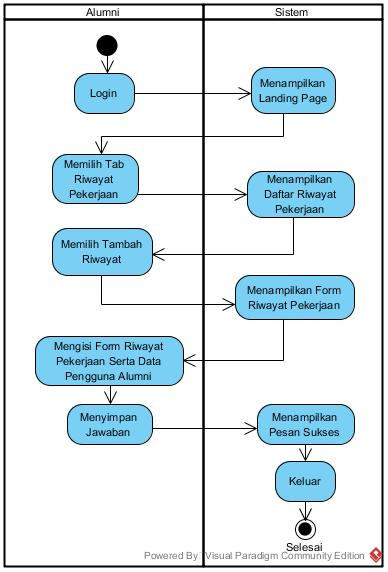
\includegraphics[width=10cm,height=15cm]{gambar/Activityriwayatpekerjaan}
	\caption{\emph{Activity Diagram} Mengisi Riwayat Pekerjaan Alumni}
	\label{activity_pekerjaanalumni}
\end{figure}

Pada sistem \textit{tracer study} ini pengguna alumni juga dapat mengisi kuesioner. Alur dari aktivitas pengisian kuesioner oleh pengguna alumni dapat dilihat pada gambar berikut.

\begin{figure}[H]
	\centering
	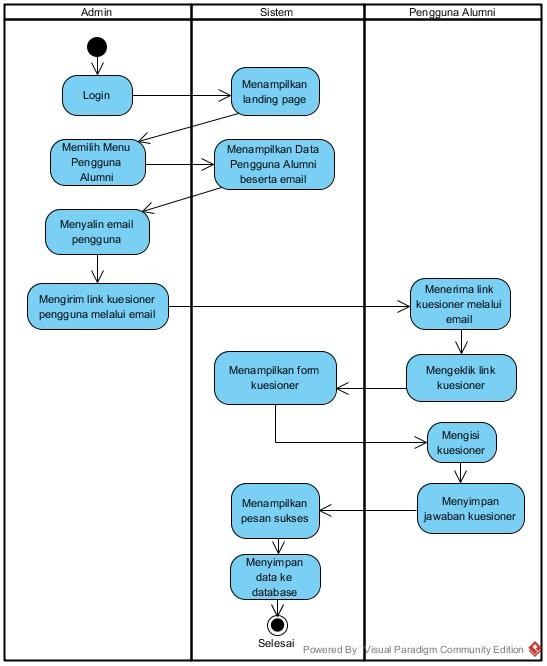
\includegraphics[width=12cm,height=14cm]{gambar/Activitykuesionerpengguna}
	\caption{\emph{Activity Diagram} Mengisi Kuesioner Pengguna Alumni}
	\label{activity_kuesionerpengguna}
\end{figure}

\begin{figure}[H]
	\centering
	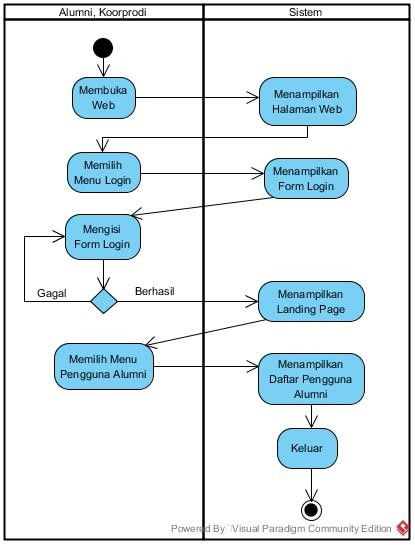
\includegraphics[width=10cm,height=11cm]{gambar/Activitymelihatpengguna}
	\caption{\emph{Activity Diagram} Melihat Daftar Pengguna Alumni}
	\label{activity_kuesionerpengguna}
\end{figure}

Alumni dan koorprodi dapat melihat daftar pengguna alumni, alur dari aktivitas tersebut dapat dilihat pada diagram di atas. Alumni dan koorprodi juga dapat melihat siapa saja alumni yang bekerja pada setiap pengguna alumni. 

\subsection{Rancangan Antar Muka Program}

Rancangan antar muka atau desain tampilan sistem dapat disebut sebagai \textit{mock-up}. Tampilan awal sistem akan memampilkan halaman pengunjung dimana disediakan menu daftar pengguna alumni dan statistik alumni. Di bawah ini adalah \textit{mock-up} untuk tampilan daftar pengguna alumni dimana pengunjung dapat melihat daftar pengguna alumni Ilmu Komputer beserta posisi alumni yang bekerja di intansi tersebut. 

\begin{figure}[H]
	\centering
	\fbox{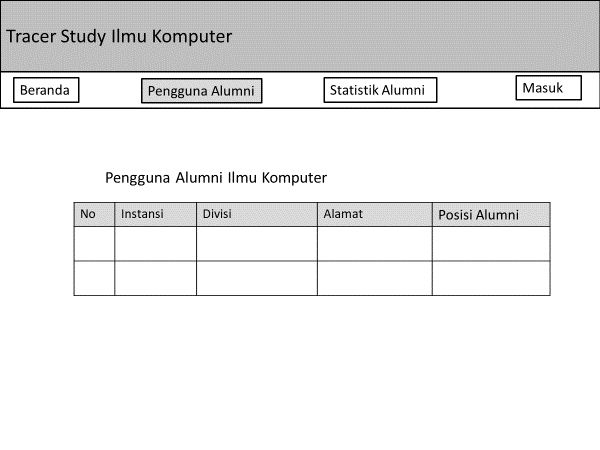
\includegraphics[width=12cm,height=10cm]{gambar/mockup/pengunjung_daftarpengguna}}
	\caption{Desain Halaman Daftar Pengguna Alumni untuk Pengunjung}
	\label{pengunjung_daftarpengguna}
\end{figure}

Sistem juga menyediakan halaman statistik alumni untuk menampilkan data \textit{tracer} yang dapat dilihat oleh pengunjung. Rancangan dari tampilan halaman tersebut dapat dilihat di bawah ini.

\begin{figure}[H]
	\centering
	\fbox{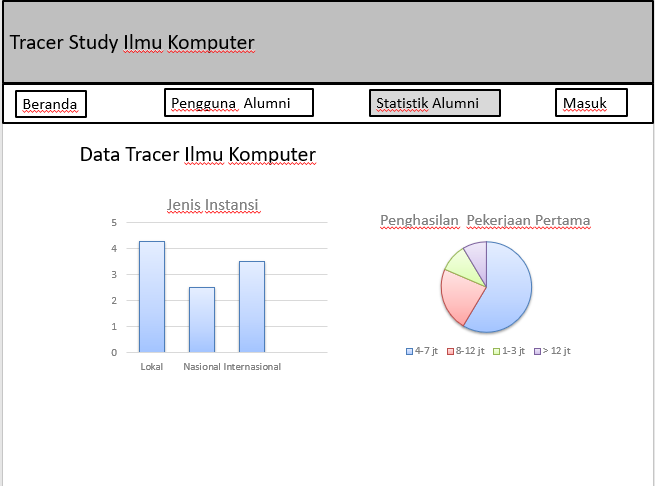
\includegraphics[width=12cm,height=9cm]{gambar/mockup/pengunjung_statistik}}
	\caption{Desain Halaman Statistik Alumni untuk Pengunjung}
	\label{pengunjung_statistik}
\end{figure}

Di bawah ini adalah rancangan tampilan dari halaman admin. Pada tampilan admin terdapat beberapa menu yaitu, beranda, alumni, pengguna alumni, kuesioner, laporan, kelola beranda, dan ganti \textit{password}. 

\begin{figure}[H]
	\centering
	\fbox{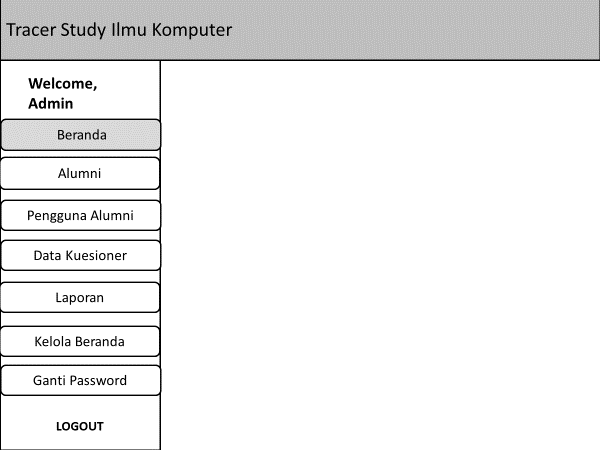
\includegraphics[width=11cm,height=8cm]{gambar/mockup/admin_beranda}}
	\caption{Desain Halaman Admin}
	\label{admin_beranda}
\end{figure}

Admin dapat mengelola data alumni dan pengguna alumni. Berikut ini rancangan tampilan dari kedua halaman tersebut. 

\begin{figure}[H]
	\centering
	\fbox{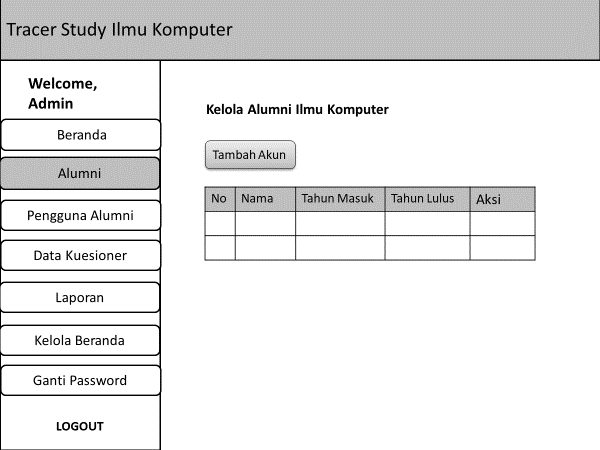
\includegraphics[width=11cm,height=8cm]{gambar/mockup/admin_kelolaalumni}}
	\caption{Desain Halaman Kelola Data Alumni}
	\label{admin_kelolaalumni}
\end{figure}

\begin{figure}[H]
	\centering
	\fbox{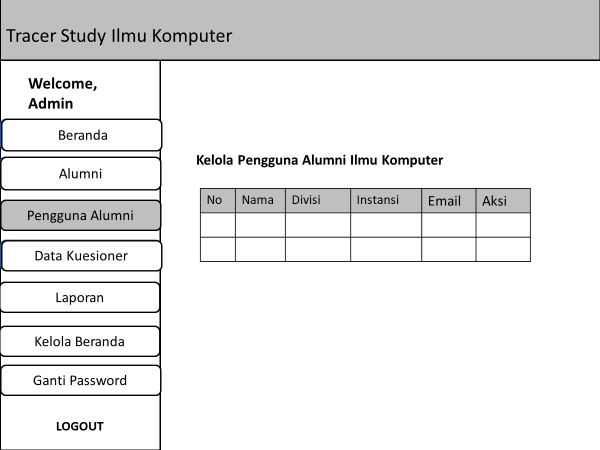
\includegraphics[width=11cm,height=8cm]{gambar/mockup/admin_kelolapengguna}}
	\caption{Desain Halaman Kelola Data Pengguna Alumni}
	\label{admin_kelolapengguna}
\end{figure}

Untuk mengelola kuesioner baik kuesioner alumni dan pengguna alumni dapat dilakukan pada halaman kelola kuesioner dibawah ini. 

\begin{figure}[H]
	\centering
	\fbox{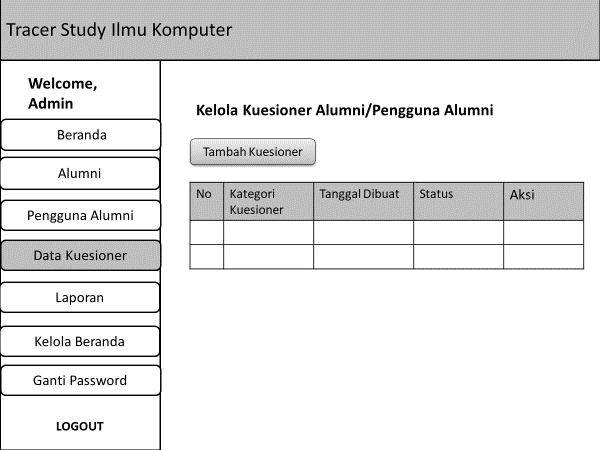
\includegraphics[width=11cm,height=8cm]{gambar/mockup/admin_kelolakuesioner}}
	\caption{Desain Halaman Kelola Kuesioner}
	\label{admin_kelolakuesioner}
\end{figure}

Gambar dibawah merupakan \textit{mock-up} dari tampilan halaman laporan tracer study. Pada halaman ini hasil \textit{tracer study} ditampilkan melalui grafik dan tabel.

\begin{figure}[H]
	\centering
	\fbox{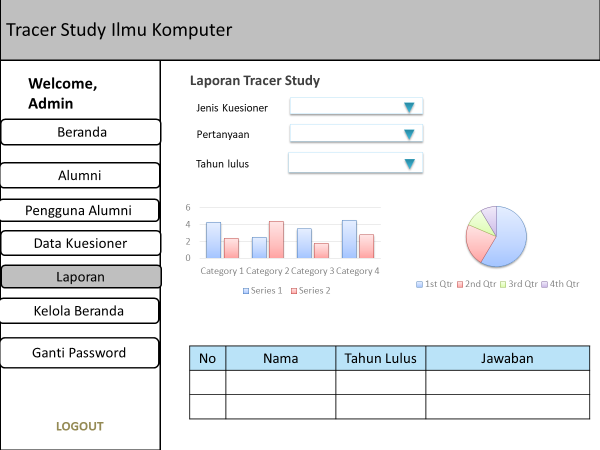
\includegraphics[width=11cm,height=8cm]{gambar/mockup/admin_laporan}}
	\caption{Desain Halaman Laporan \textit{Tracer Study}}
	\label{admin_kelolakuesioner}
\end{figure}

\begin{figure}[H]
	\centering
	\fbox{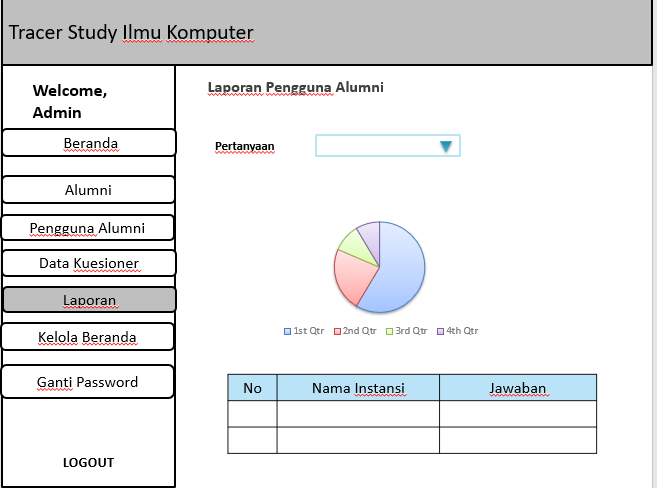
\includegraphics[width=11cm,height=8cm]{gambar/mockup/admin_laporanpengguna}}
	\caption{Desain Halaman Laporan Pengguna Alumni}
	\label{admin_laporanpengguna}
\end{figure}

Pada tampilan koorprodi terdapat beberapa menu, yaitu beranda, alumni, pengguna alumni, laporan, dan ganti password. 

\begin{figure}[H]
	\centering
	\fbox{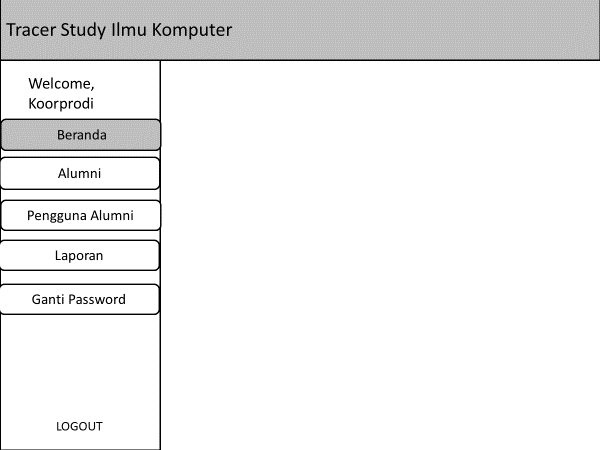
\includegraphics[width=11cm,height=8cm]{gambar/mockup/koorprodi_beranda}}
	\caption{Desain Halaman Koorprodi}
	\label{koorprodi_beranda}
\end{figure}

\begin{figure}[H]
	\centering
	\fbox{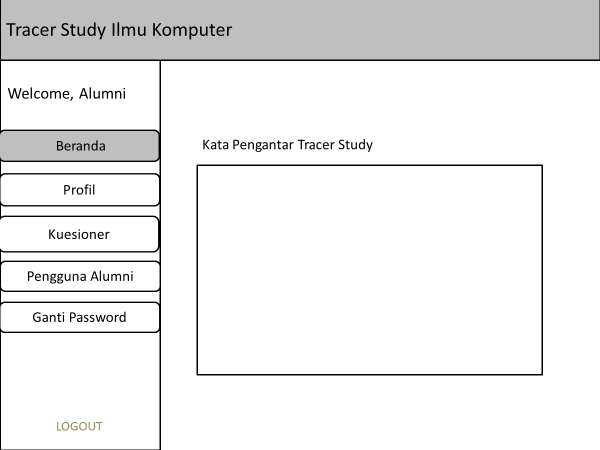
\includegraphics[width=11cm,height=8cm]{gambar/mockup/alumni_beranda}}
	\caption{Desain Halaman Alumni}
	\label{alumni_beranda}
\end{figure}

Selanjutnya beralih ke halaman alumni dimana terdapat beberapa menu, yaitu beranda yang terdiri dari form pengisian data \textit{tracer study} yaitu data diri, pekerjaan dan kuesioner, kemudian menu pengguna alumni, dan menu ganti \textit{password}. Rancangan tampilan halaman alumni dapat dilihat pada gambar 3.19. Alumni dapat mengisi kuesioner melalui halaman kuesioner. Berikut rancangan tampilan dari halaman kuesioner alumni.

\begin{figure}[H]
	\centering
	\fbox{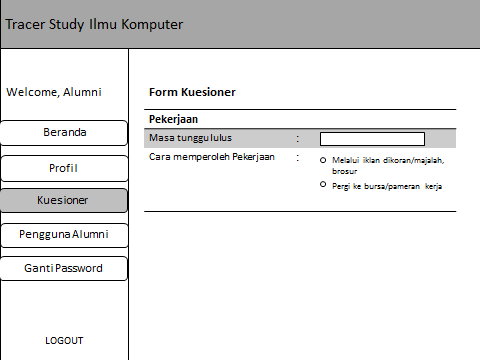
\includegraphics[width=11cm,height=8cm]{gambar/mockup/alumni_kuesioner}}
	\caption{Desain Halaman Kuesioner Alumni}
	\label{alumni_beranda}
\end{figure}

Selanjutnya sistem menyediakan tampilan daftar pengguna alumni yang dapat dilihat alumni beserta siapa saja alumni yang bekerja pada instansi dari pengguna alumni terkait.\textit{ Mock-up} dari tampilan daftar pengguna alumni dapat dilihat sebagai berikut.

\begin{figure}[H]
	\centering
	\fbox{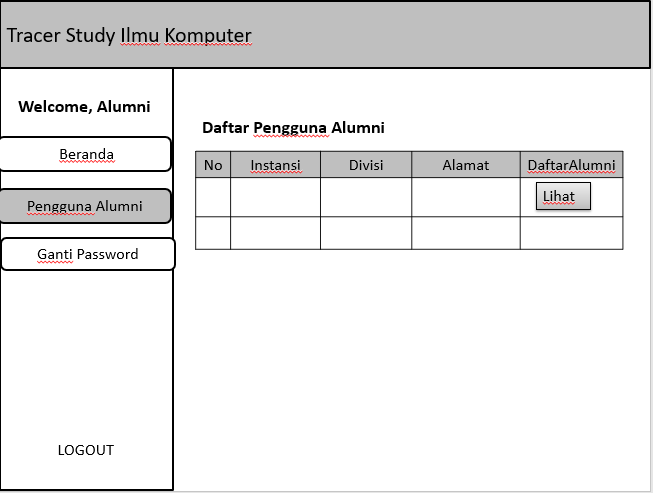
\includegraphics[width=11cm,height=8cm]{gambar/mockup/alumni_daftarpengguna}}
	\caption{Desain Halaman Daftar Pengguna Alumni untuk Alumni}
	\label{alumni_beranda}
\end{figure}

\section{Pengembangan}
Tahap pengembangan atau juga disebut tahap konstruksi merupakan tahapan dimana menuangkan seluruh desain yang telah dibuat kedalam kode program. tahapan ini dimulai dari membangun basis data, mengimplementasikan desain tampilan dan dilanjutkan dengan membangun sistem.  

\subsection{Membangun Basis Data}
Pada tahap ini dibangun basis data berdasarkan \textit{Entity Relationship Diagram} yang dibuat pada tahap sebelumnya, yaitu desain sistem. Basis data dibuat menggunakan MySQL dan memanfaatkan aplikasi phpMyAdmin untuk membuat tabel beserta relasinya. Berikut bentuk basis data Sistem Informasi \textit{Tracer Study} Prodi Ilmu Komputer yang memiliki 12 tabel:

\begin{figure}[H]
	\centering
	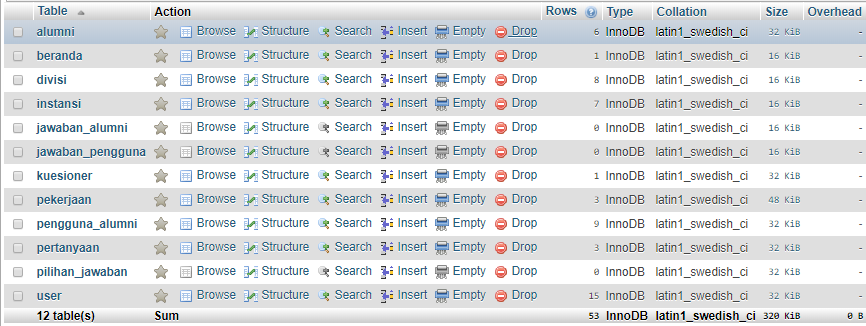
\includegraphics[width=13cm,height=7cm]{gambar/database}
	\caption{Basis Data  Sistem Informasi \textit{Tracer Study} Prodi Ilmu Komputer }
	\label{database}
\end{figure}

\subsection{Implementasi Desain Tampilan}
Untuk mengimplentasikan desain tampilan, digunakan \textit{Bootstrap} sebagai \textit{framework} untuk membuat tampilan atau \textit{front-end} dan CodeIgniter sebagai \textit{framework} untuk \textit{back-end}. Dengan menggunakan CodeIgniter memudahkan dalam mengimplementasikan arsitektur MVC dimana sudah disediakan struktur folder yang sesuai. \textit{Framework Bootsrap} digunakan pada bagian View. Berikut tampilan \textit{website} sistem \textit{tracer study} Ilmu Komputer yang terintegrasi dengan Sistem Informasi Alumni hasil penelitian Ibu Fariani Hermin selaku dosen Ilmu Komputer yang dapat dilihat pada \textit{browser}.

\begin{figure}[H]
	\centering
	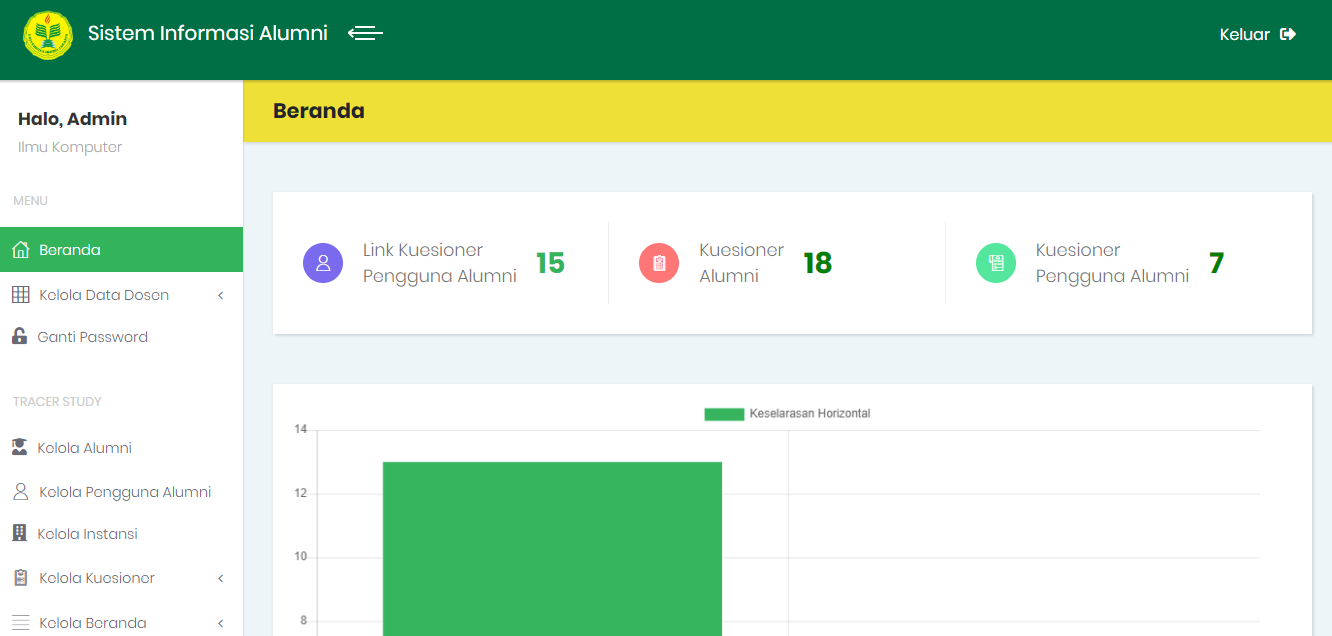
\includegraphics[width=14cm,height=7cm]{gambar/tampilan/admin_beranda}
	\caption{Tampilan Halaman Beranda Admin}
	\label{ui_adminBeranda}
\end{figure}
 
Menu \textit{tracer study} terdapat pada bagian bawah kiri seperti pada Gambar 3.23. Gambar tersebut merupakan tampilan halaman beranda admin yang berisi statistik alumni ilmu komputer, jumlah pengguna alumni yang baru terdaftar, jumlah responden kuesioner alumni dan pengguna alumni. 

\begin{figure}[H]
	\centering
	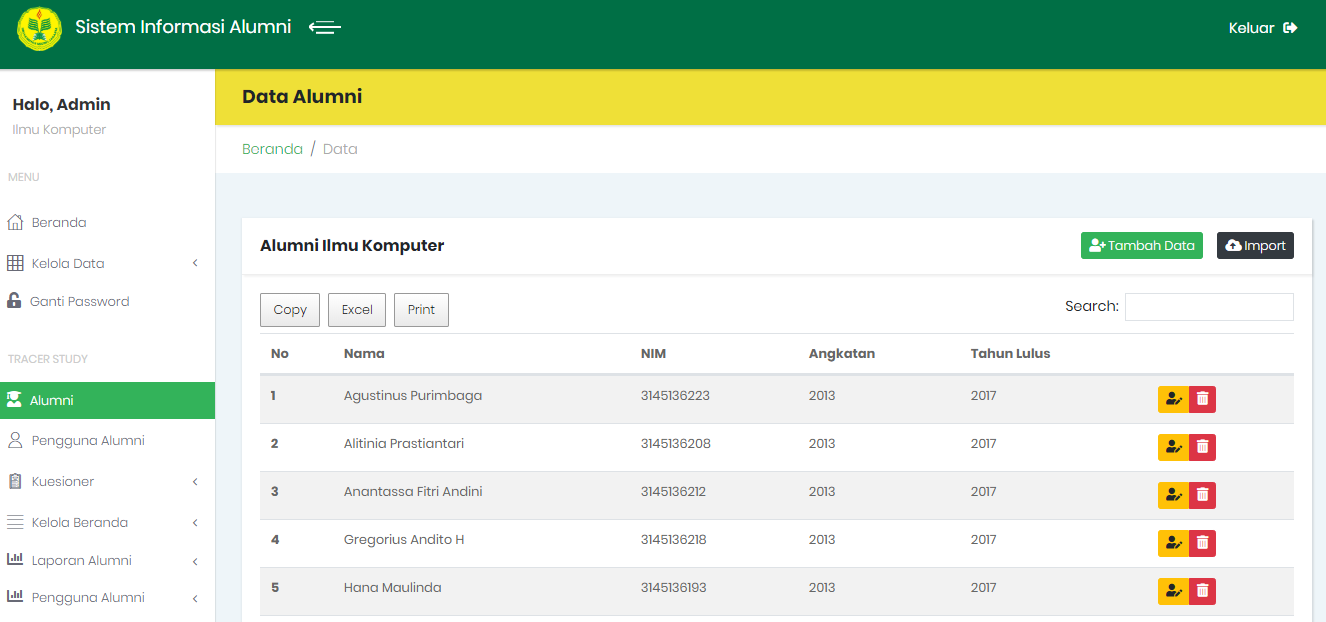
\includegraphics[width=14cm,height=7cm]{gambar/tampilan/admin_kelolaAlumni}
	\caption{Tampilan Halaman Kelola Alumni pada Admin }
	\label{ui_adminKelolaAlumni}
\end{figure}

Gambar 3.24 adalah tampilan pada admin untuk mengelola data alumni seperti tambah, sunting, hapus, dan \textit{import} data alumni.  Selanjutnya, halaman untuk mengelola data pengguna alumni pada admin. Berikut tampilan dari halaman tersebut yang dapat dilihat pada Gambar 3.25.

\begin{figure}[H]
	\centering
	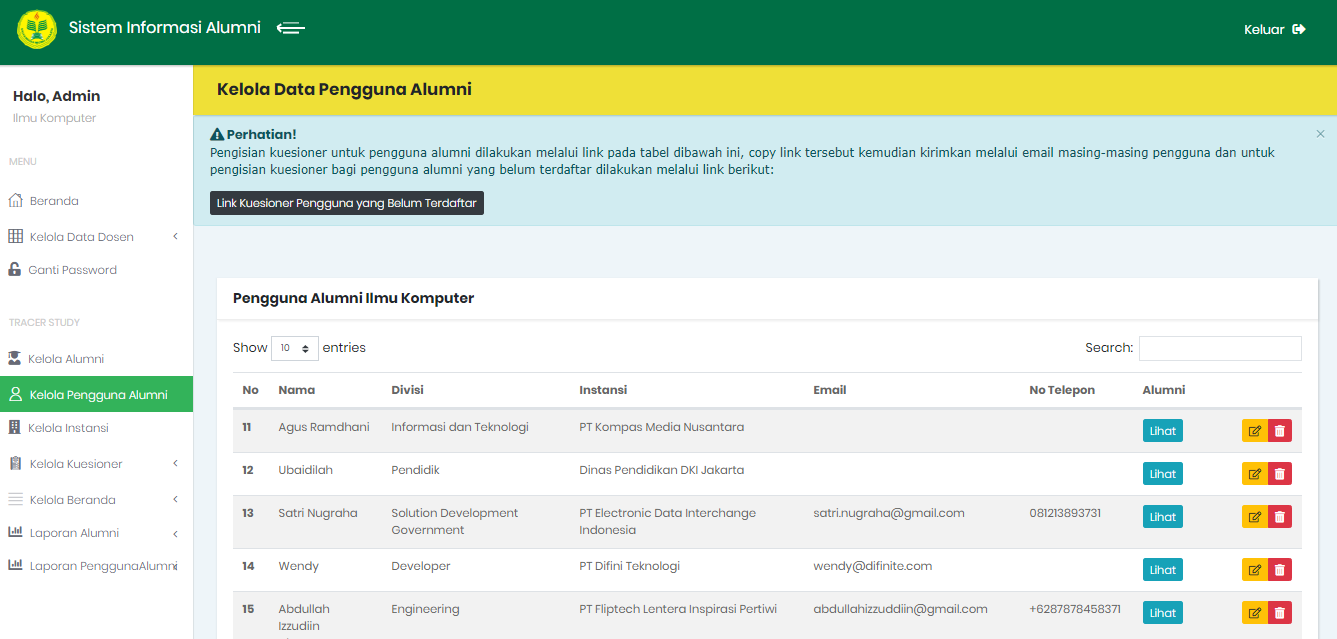
\includegraphics[width=14cm,height=7cm]{gambar/tampilan/admin_kelolaPenggunaAlumni}
	\caption{Tampilan Halaman Kelola Pengguna Alumni pada Admin }
	\label{ui_adminKelolaPenggunaAlumni}
\end{figure}

\begin{figure}[H]
	\centering
	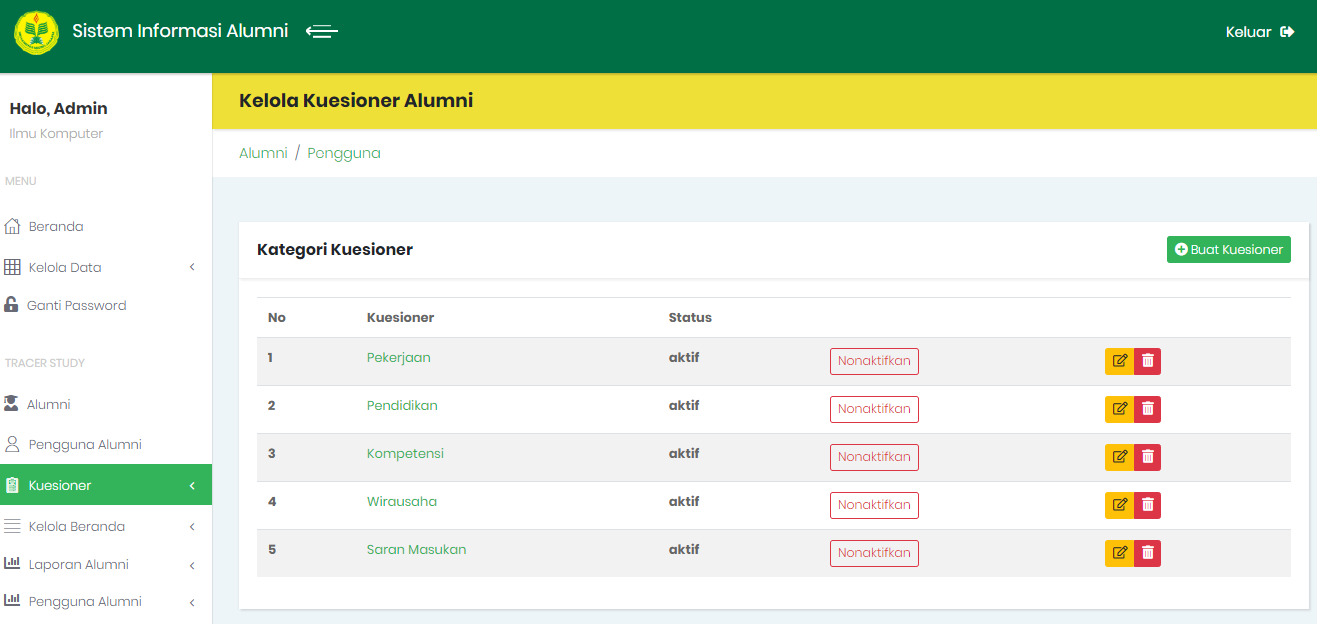
\includegraphics[width=14cm,height=7cm]{gambar/tampilan/admin_kelolaKuesioner}
	\caption{Tampilan Halaman Kelola Kuesioner Alumni pada Admin }
	\label{ui_adminkelolaKuesionerAlumni}
\end{figure}

Gambar 3.26 merupakan tampilan pada admin yang ditujukan untuk mengelola kuesioner-kuesioner alumni. Pada halaman ini tersedia fitur untuk menambah, menyunting, menghapus kuesioner dan dapat mengaktifkan serta menonaktifkan kuesioner. 

\begin{figure}[H]
	\centering
	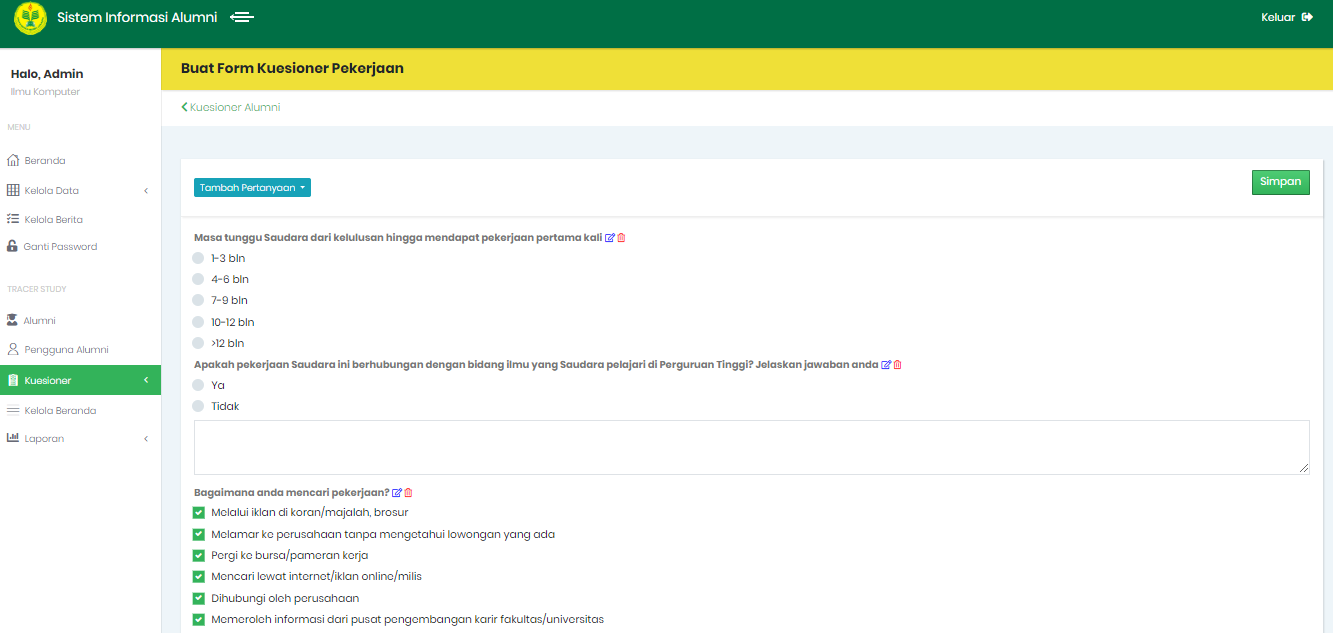
\includegraphics[width=14cm,height=7cm]{gambar/tampilan/admin_buatKuesioner}
	\caption{Tampilan Halaman Buat Kuesioner Alumni pada Admin }
	\label{ui_adminBuatKuesionerAlumni}
\end{figure}

Jika admin memilih tombol buat kuesioner maka sistem akan menampilkan halaman buat kuesioner seperti pada Gambar 3.27. Pada halaman tersebut admin dapat membuat empat jenis pertanyaan, yaitu isian, pertanyaan dengan jawaban pilihan, pertanyaan dengan jawaban lebih dari satu atau ganda, dan pertanyaan dengan jawaban menggunakan skala penilaian.

%penjelasan dan gambar halaman buat kuesioner pengguna
\begin{figure}[H]
	\centering
	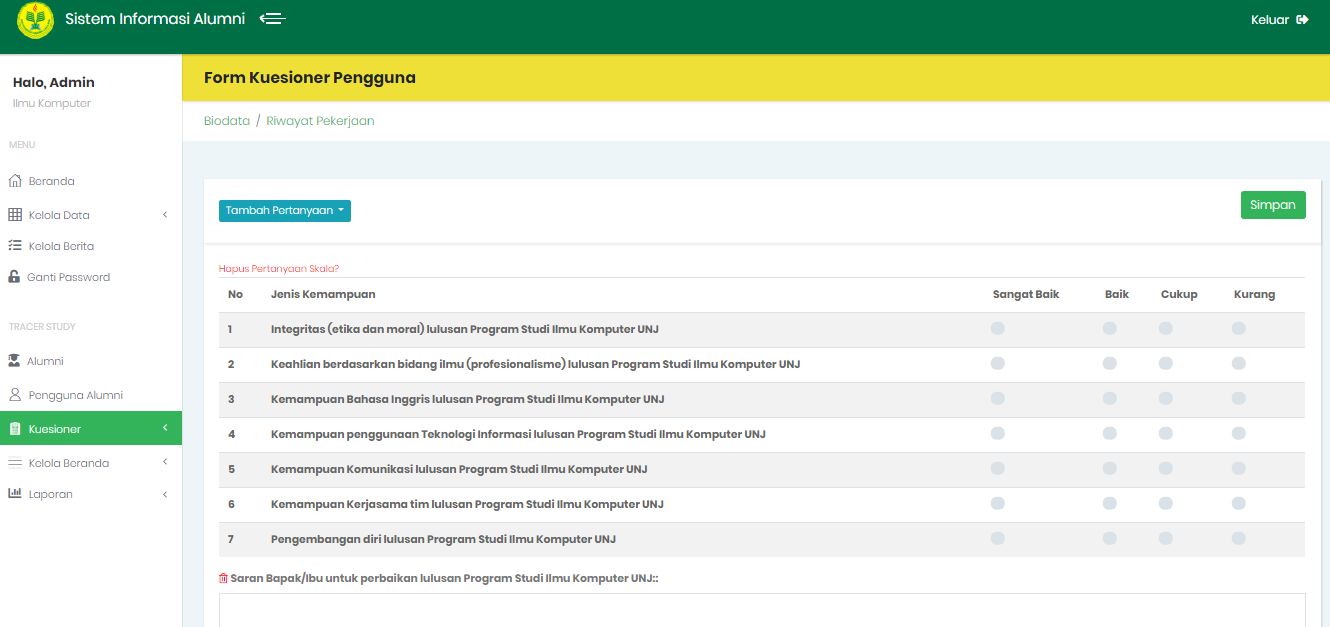
\includegraphics[width=14cm,height=7cm]{gambar/tampilan/admin_buatKuesionerPengguna}
	\caption{Tampilan Halaman Buat Kuesioner Pengguna pada Admin }
	\label{ui_adminBuatKuesionerPenggunaAlumni}
\end{figure}

Selain membuat form kuesioner untuk alumni, admin juga dapat membuat form kuesioner untu pengguna alumni. Tampilan halaman buat form kuesioner pengguna alumni dapat dilihat pada Gambar 3.28. 

\begin{figure}[H]
	\centering
	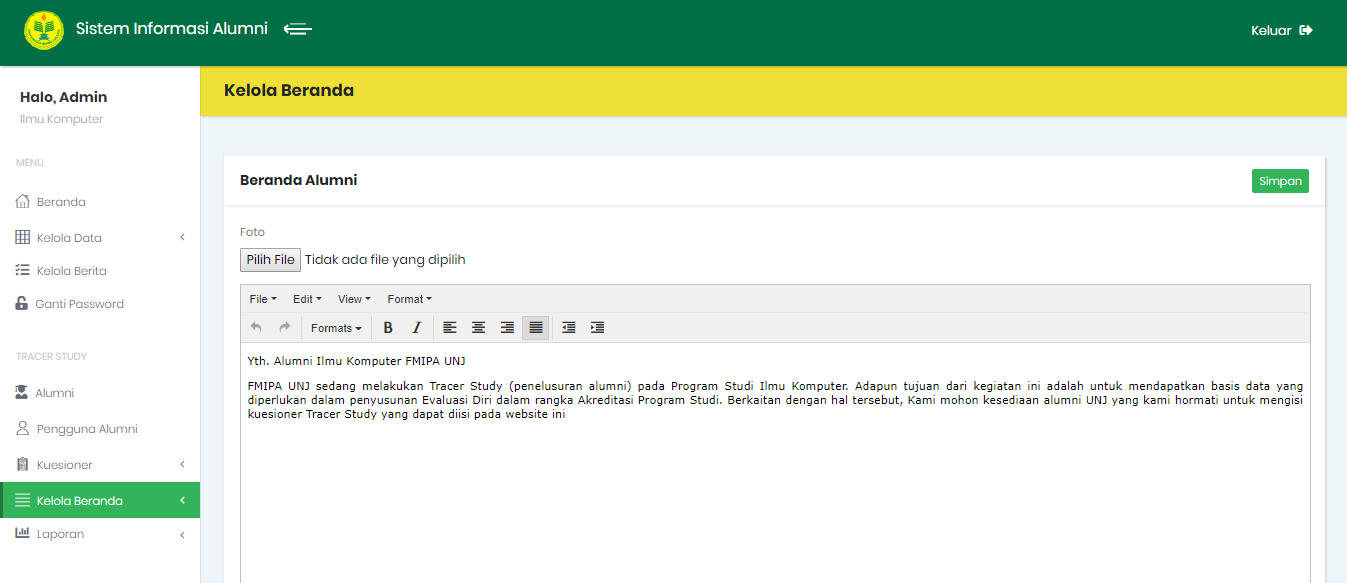
\includegraphics[width=14cm,height=7cm]{gambar/tampilan/admin_kelolaBerandaAlumni}
	\caption{Tampilan Halaman Kelola Beranda Alumni pada Admin }
	\label{ui_adminKelolaBerandaAlumni}
\end{figure}

Pada pengembangan sistem ini juga disediakan fitur untuk mengelola kata pengantar pada beranda alumni agar dapat menyesuaikan jika ada perubahan dari pihak prodi di masa mendatang. Fitur tersebut terdapat pada menu kelola beranda yang tampilannya dapat dilihat pada Gambar 3.29. 

\begin{figure}[H]
	\centering
	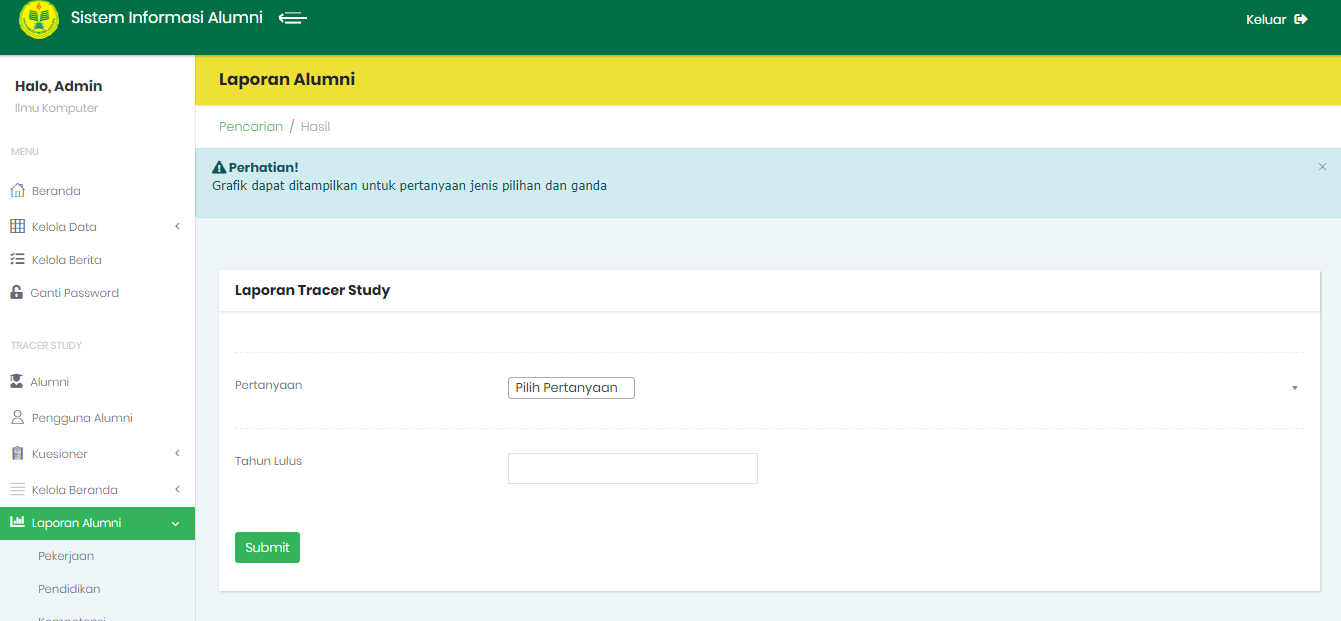
\includegraphics[width=14cm,height=7cm]{gambar/tampilan/admin_cariLaporan}
	\caption{Tampilan Halaman Kriteria Laporan Alumni pada Admin }
	\label{ui_adminCariLaporan}
\end{figure}

\begin{figure}[H]
	\centering
	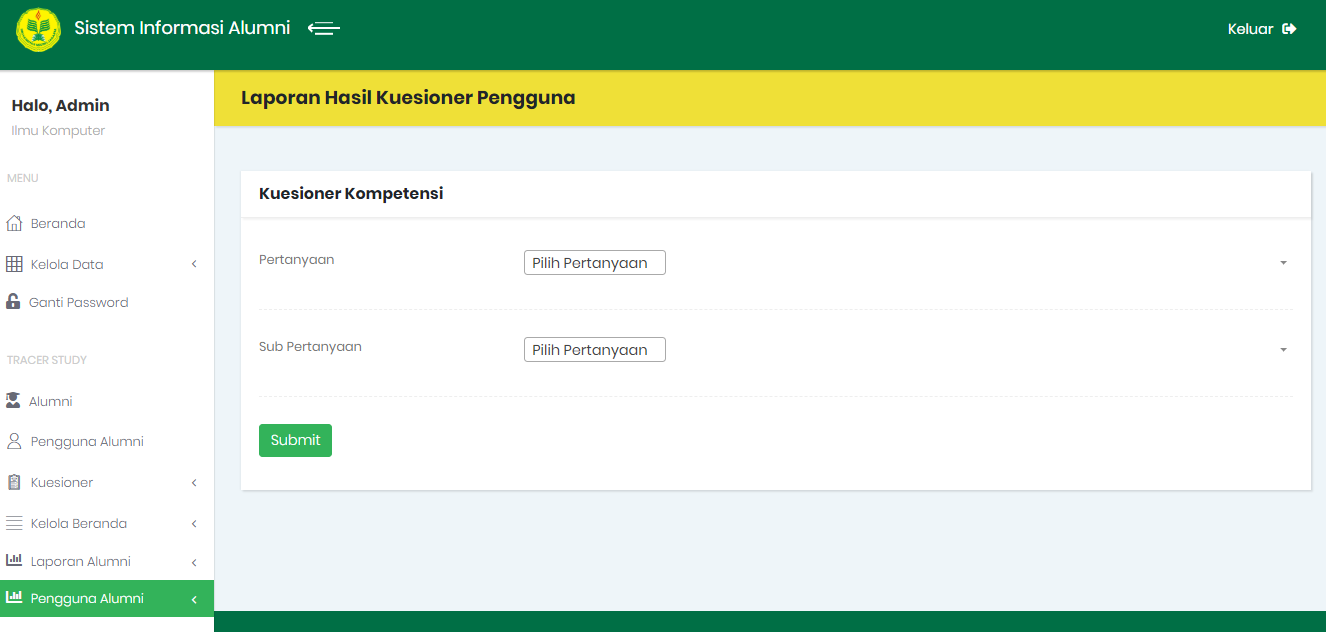
\includegraphics[width=14cm,height=7cm]{gambar/tampilan/admin_cariLaporanPengguna}
	\caption{Tampilan Halaman Kriteria Laporan Pengguna Alumni pada Admin }
	\label{ui_adminCariLaporanPengguna}
\end{figure}

Gambar 3.30 dan Gambar 3.31 merupakan tampilan halaman kriteria laporan atau hasil \textit{tracer study} alumni dan pengguna alumni. Sebelum menampilkan halaman hasil \textit{tracer study}, admin harus memilih terlebih dahulu kriteria laporan yang ingin dilihat, yaitu berupa pertanyaan dan tahun lulus. Setelah admin memilih kriteria maka sistem akan menampilkan halaman hasil \textit{tracer study} berupa grafik dan tabel yang dapat dilihat pada gambar berikut. 

%gambar hasil tracer study Gambar 3.32

\begin{figure}[H]
	\centering
	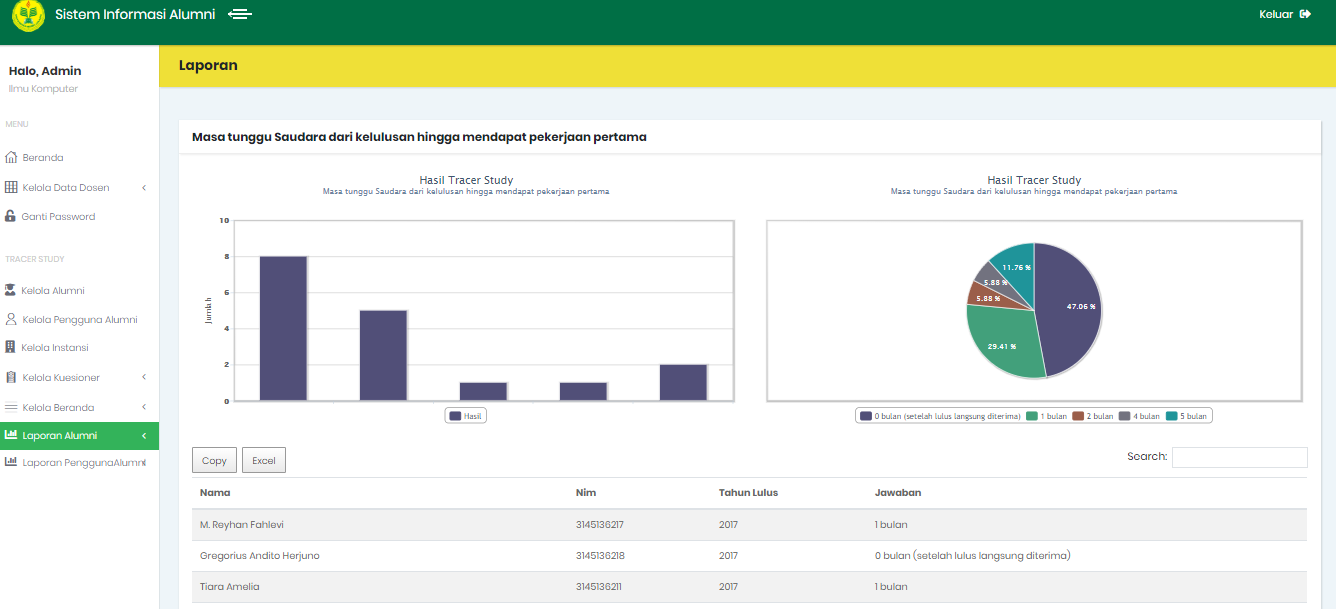
\includegraphics[width=14cm,height=7cm]{gambar/tampilan/admin_hasilLaporanAlumni}
	\caption{Tampilan Halaman Hasil \textit{Tracer Study} pada Admin dan Koorprodi}
	\label{ui_adminHasilLaporanAlumni}
\end{figure}

\begin{figure}[H]
	\centering
	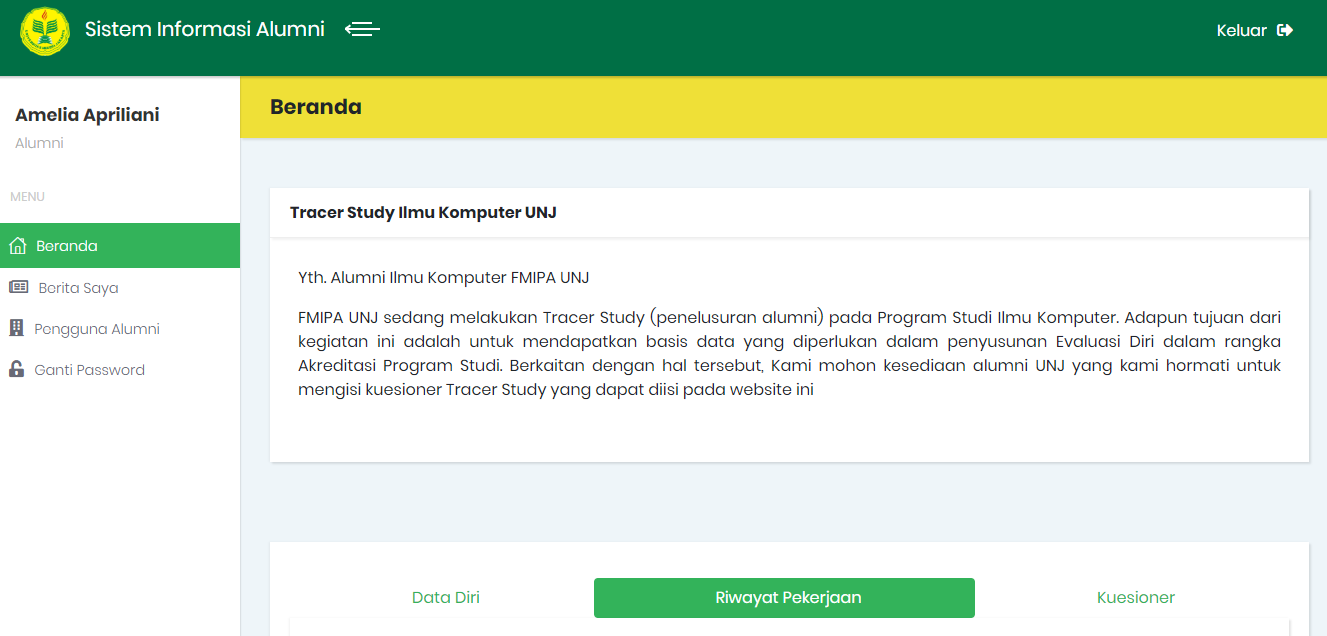
\includegraphics[width=14cm,height=7cm]{gambar/tampilan/alumni_beranda}
	\caption{Tampilan Halaman Beranda pada Alumni }
	\label{ui_alumniBeranda}
\end{figure}

Selanjutnya halaman alumni, setelah alumni melakukan \textit{login} sistem akan menampilkan halaman beranda alumni yang dapat dilihat pada Gambar 3.33. Beranda alumni berisi kata pengantar \textit{tracer study} yang dapat disunting oleh admin serta pengisian data \textit{tracer study} yang terdiri dari data diri, pekerjaan, dan kuesioner.  

\begin{figure}[H]
	\centering
	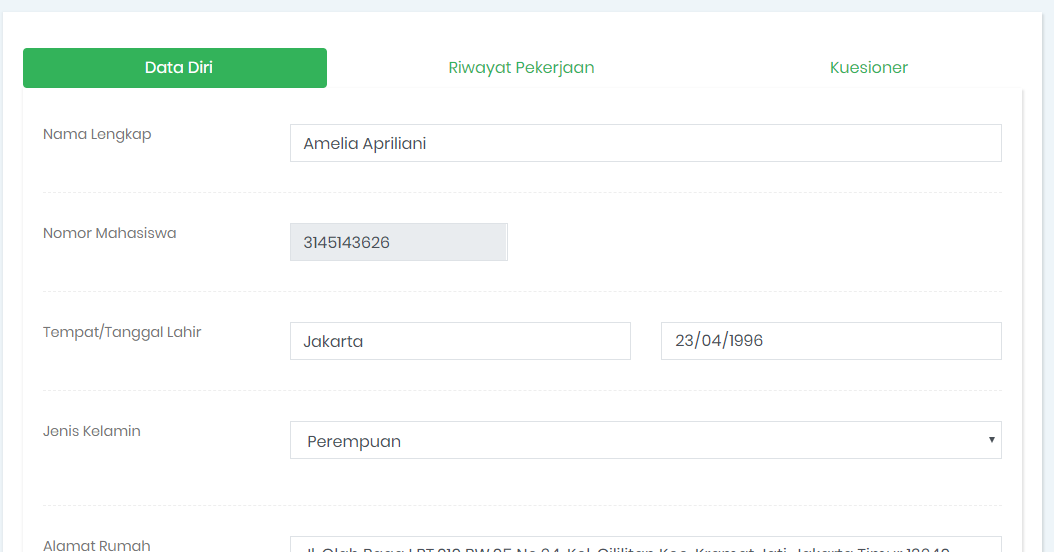
\includegraphics[width=14cm,height=7cm]{gambar/tampilan/alumni_profil}
	\caption{Tampilan Halaman Data Diri pada Alumni }
	\label{ui_alumniProfil}
\end{figure}

\begin{figure}[H]
	\centering
	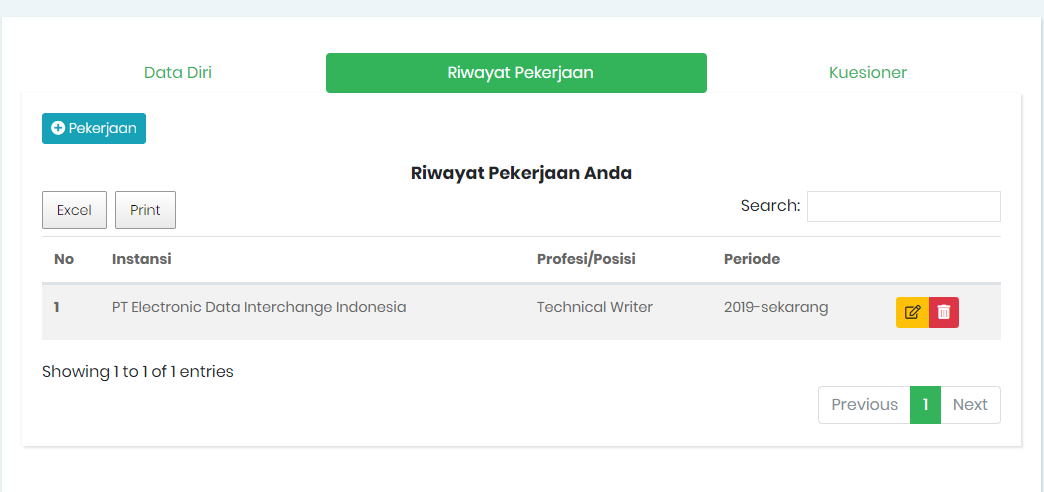
\includegraphics[width=14cm,height=7cm]{gambar/tampilan/alumni_pekerjaan}
	\caption{Tampilan Halaman Form Riwayat Pekerjaan pada Alumni }
	\label{ui_alumniInputPekerjaan}
\end{figure}

Gambar 3.34 adalah tampilan untuk melengkapi data diri alumni. Sedangkan gambar 3.35 merupakan tampilan form untuk memasukan data riwayat pekerjaan alumni

\begin{figure}[H]
	\centering
	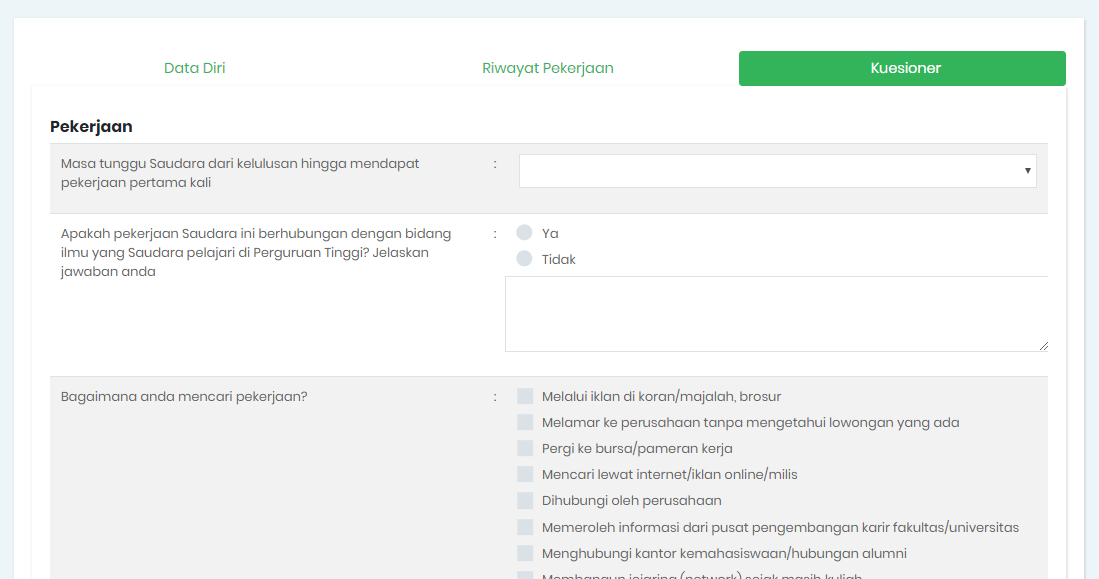
\includegraphics[width=14cm,height=7cm]{gambar/tampilan/alumni_kuesioner}
	\caption{Tampilan Halaman Kuesioner pada Alumni }
	\label{ui_alumniKuesioner}
\end{figure}

Gambar 3.36 adalah tampilan halaman mengisi kuesioner untuk alumni. Semua jenis kuesioner ditampilkan dalam satu halaman. Halaman kuesioner ini menyediakan pertanyaan isian, pilihan, ganda atau dapat memilih lebih dari satu jawaban, dan pertanyaan dengan skala penilaian.


\begin{figure}[H]
	\centering
	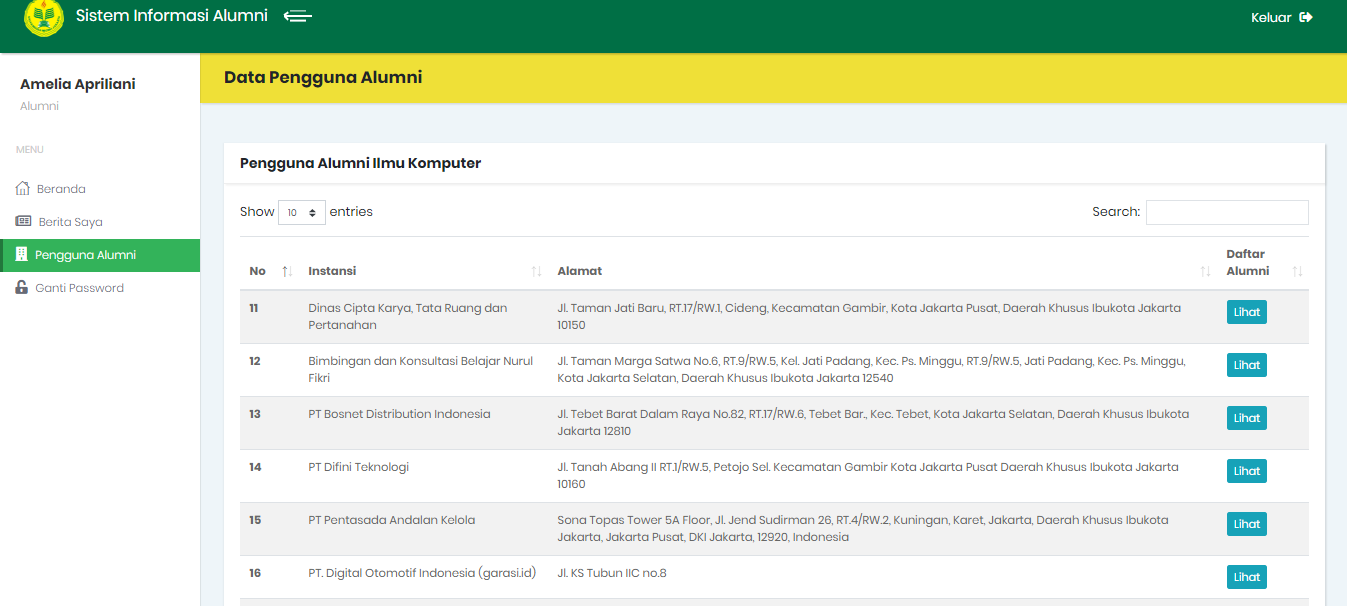
\includegraphics[width=14cm,height=7cm]{gambar/tampilan/alumni_daftarPengguna}
	\caption{Tampilan Halaman Daftar Pengguna pada Alumni }
	\label{ui_alumniDaftarPengguna}
\end{figure}

\begin{figure}[H]
	\centering
	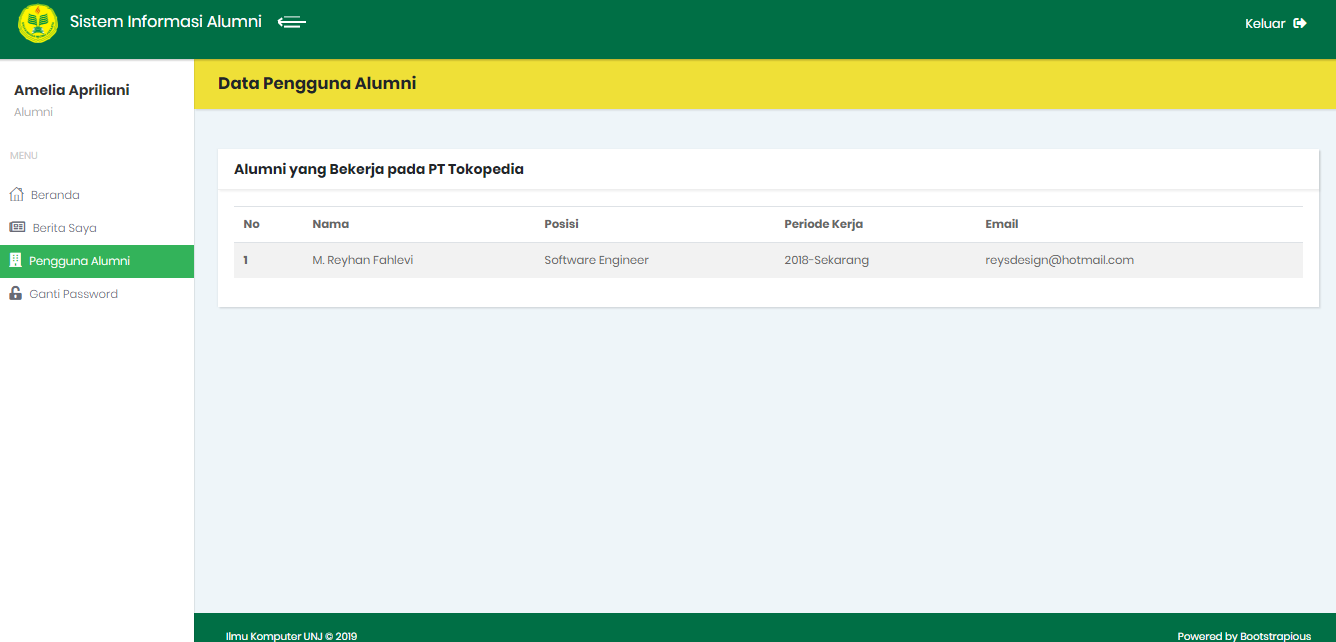
\includegraphics[width=14cm,height=7cm]{gambar/tampilan/alumni_alumniPengguna}
	\caption{Tampilan Halaman Daftar Pengguna pada Alumni }
	\label{ui_alumniPengguna}
\end{figure}

Pada pengembangan sistem ini menyediakan fasilitas untuk berbagi informasi antar alumni dapat dilihat pada Gambar 3.37 dan Gambar 3.38. Gambar 3.37 merupakan halaman daftar pengguna alumni pada alumni. Pada halaman ini alumni dapat melihat daftar pengguna alumni dari prodi Ilmu Komputer. Jika alumni memilih tombol lihat pada kolom daftar alumni, sistem akan menampilkan halaman daftar alumni yang bekerja pada pengguna alumni terkait seperti pada Gambar 3.38. 

\begin{figure}[H]
	\centering
	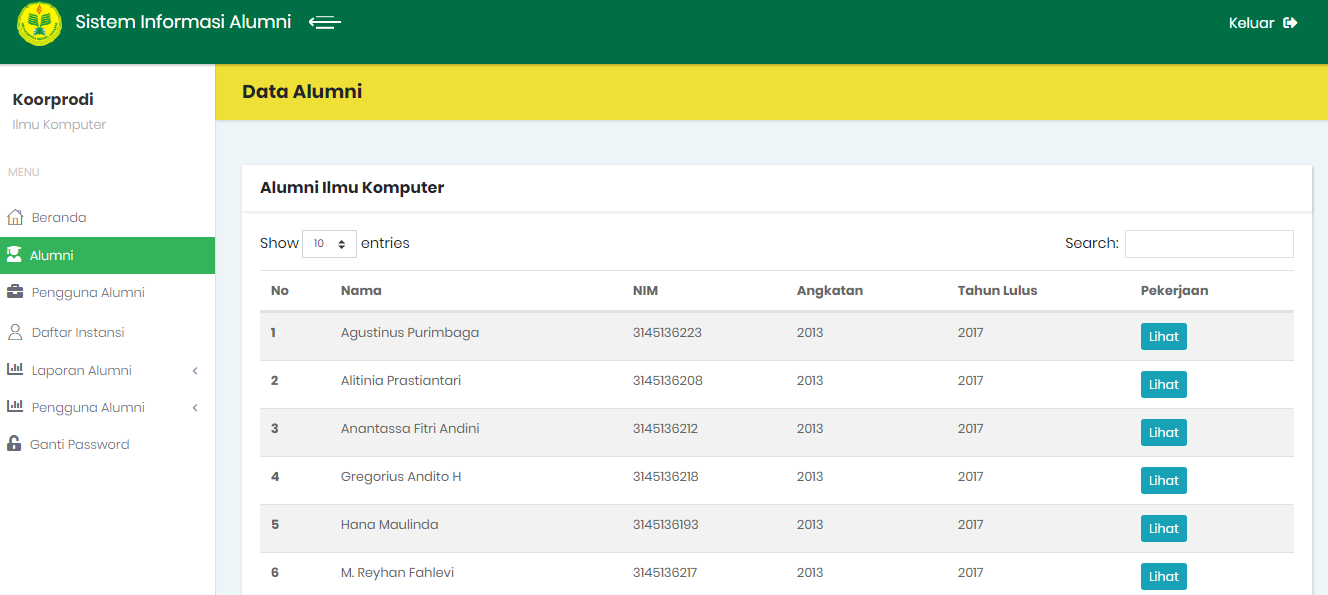
\includegraphics[width=14cm,height=7cm]{gambar/tampilan/koorprodi_daftarAlumni}
	\caption{Tampilan Halaman Daftar Alumni pada Koorprodi }
	\label{ui_koorprodiDaftarAlumni}
\end{figure}

Selanjutnya halaman untuk koorprodi. Halaman koorprodi dapat dilihat pada Gambar 3.39. Halaman koorprodi menyediakan menu untuk melihat data alumni beserta pekerjaannya, menu untuk melihat daftar pengguna alumni, menu untuk melihat daftar instansi beserta skala instansi dan menu untuk halaman laporan hasil \textit{tracer study}. 

\begin{figure}[H]
	\centering
	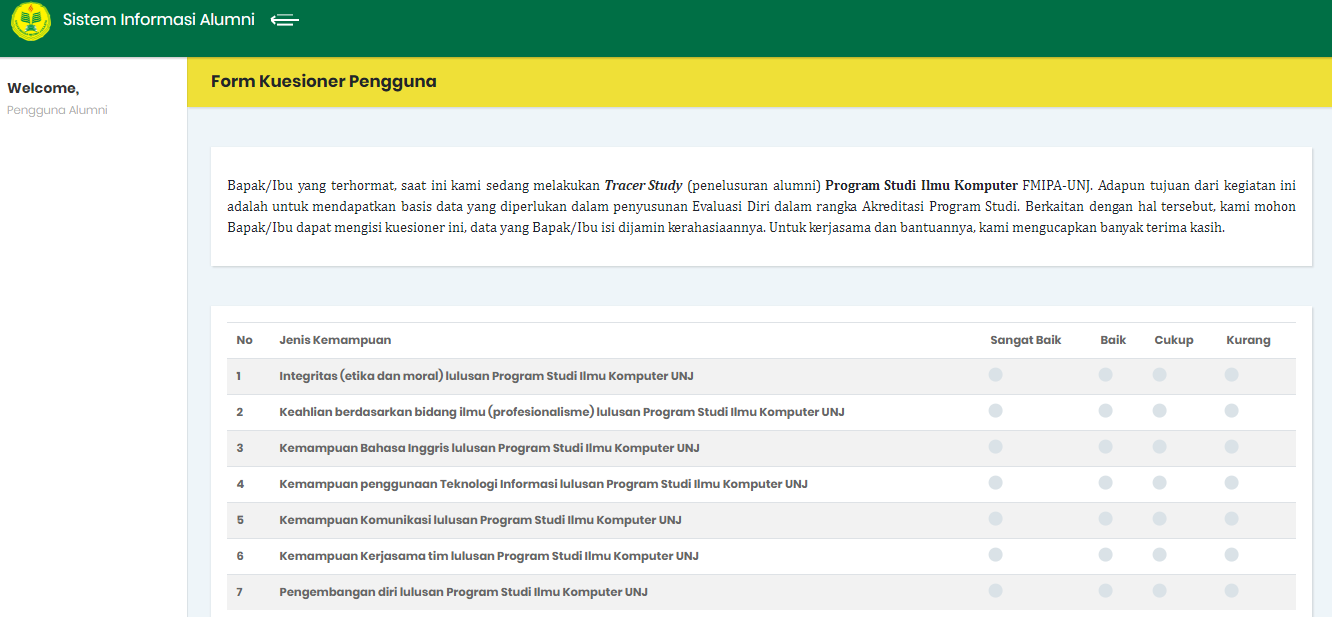
\includegraphics[width=14cm,height=7cm]{gambar/tampilan/penggunaAlumni_kuesioner}
	\caption{Tampilan Halaman Kuesioner untuk Pengguna Alumni}
	\label{ui_penggunaAlumniKuesioner}
\end{figure}

Gambar 3.40 merupakan halaman kuesioner yang diperuntukkan untuk pengguna alumni. Halaman ini akan muncul setelah pengguna alumni mengklik \textit{link} kuesioner yang dikirimkan admin melalui \textit{email}. 

\begin{figure}[H]
	\centering
	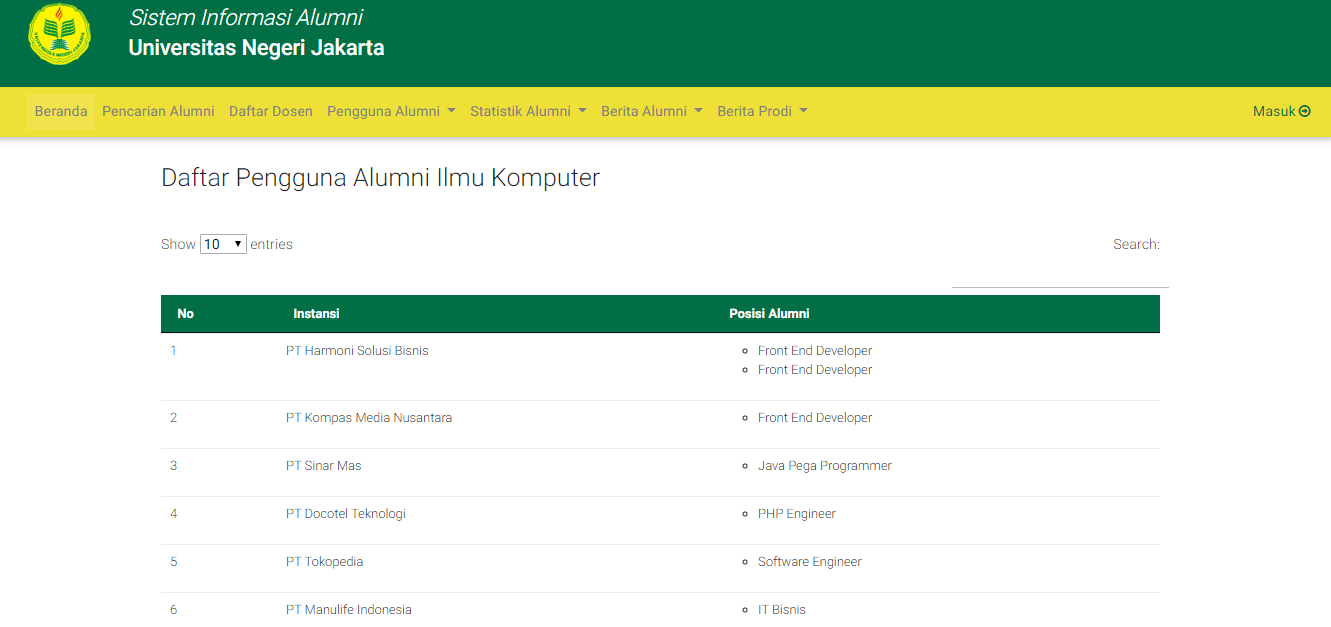
\includegraphics[width=14cm,height=7cm]{gambar/tampilan/pengunjung_daftarPengguna}
	\caption{Tampilan Halaman Daftar Pengguna Alumni untuk Pengunjung}
	\label{ui_pengunjungDaftarPengguna}
\end{figure}

\begin{figure}[H]
	\centering
	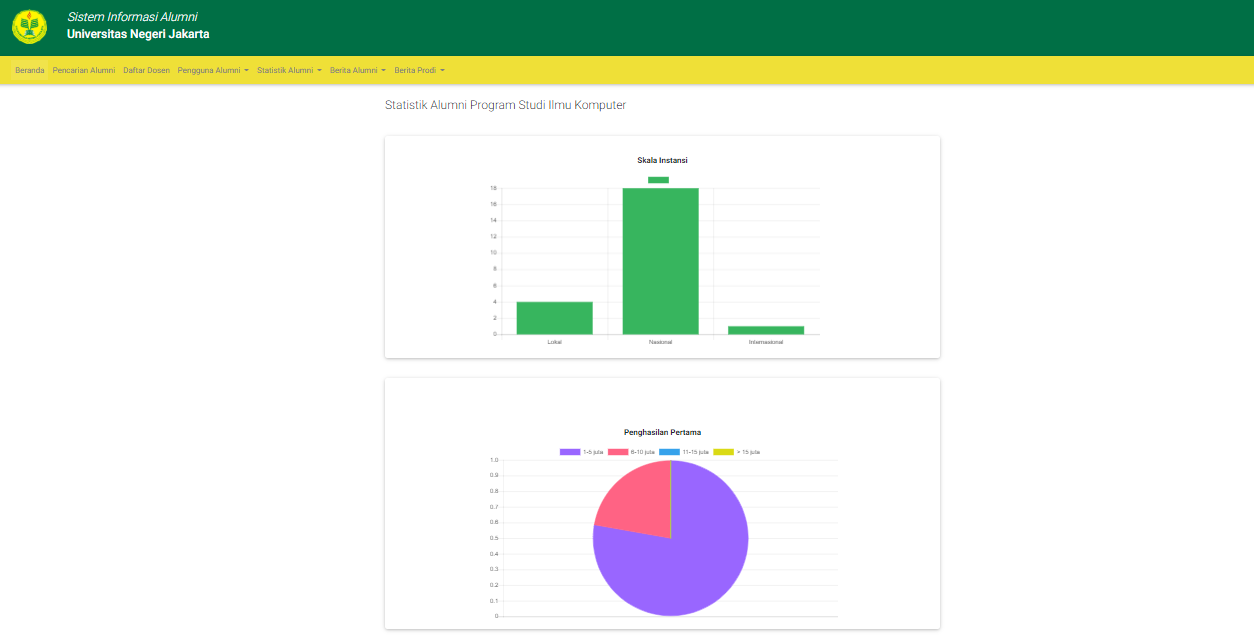
\includegraphics[width=14cm,height=7cm]{gambar/tampilan/pengunjung_statistik}
	\caption{Tampilan Halaman Statistik Alumni untuk Pengunjung}
	\label{ui_pengunjungStatistik}
\end{figure}

Selanjutnya adalah tampilan halaman yang dapat dilihat oleh pengunjung \textit{website} tanpa \textit{login}, yaitu terdapat halaman daftar pengguna alumni yang dapat dilihat pada Gambar 3.41 dan halaman statistik alumni yang dapat dilihat pada Gambar 3.42. Halaman daftar pengguna alumni berisi instansi-instansi tempat alumni bekerja beserta posisi pekerjaan alumni pada instansi terkait. Sedangkan halaman statistik alumni berisi beberapa hasil \textit{tracer study} yang dapat dilihat pengunjung.

\subsection{Implementasi Sistem (\textit{Back End})}
Dalam pengimplementasian semua fungsi yang berada dalam sistem digunakan bahasa pemrograman PHP kemudian menggunakan \textit{framework codeIgniter} untuk memudahkan dalam mengimplementasikan arsitektur MVC. Dengan arsitektur MVC proses pengkodean dibagi menjadi tiga bagian, yaitu Model untuk menyimpan fungsi yang berhubungan dengan \textit{database}, kemudian View untuk menampilkan informasi yang direpresentasikan kepada pengguna, dan Controller yang menjembatani antara Model dan View. Berikut merupakan sampel pemrograman terdiri dari \textit{Model}, \textit{View}, dan \textit{Controller}.

\begin{figure}[H]
	\centering
	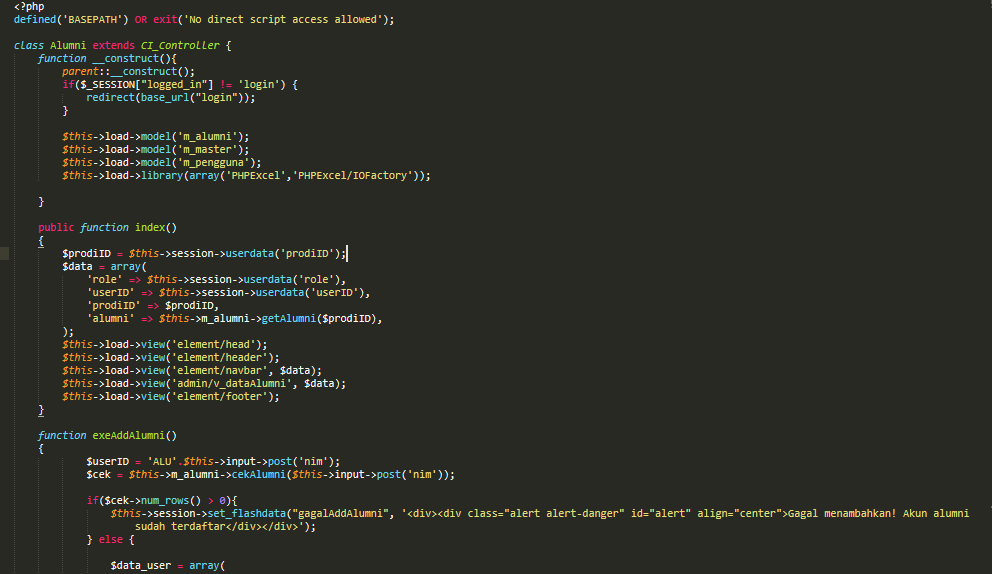
\includegraphics[width=14cm,height=7cm]{gambar/source_code/c_alumni}
	\caption{Struktur Pemrograman \textit{Controller}}
	\label{sc_cAlumni}
\end{figure}

\begin{figure}[H]
	\centering
	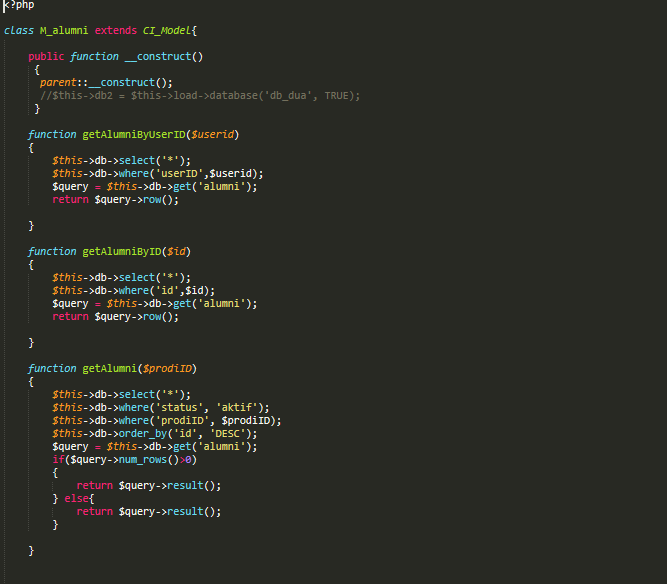
\includegraphics[width=14cm,height=7cm]{gambar/source_code/m_alumni}
	\caption{Struktur Pemrograman \textit{Model}}
	\label{sc_mAlumni}
\end{figure}

\begin{figure}[H]
	\centering
	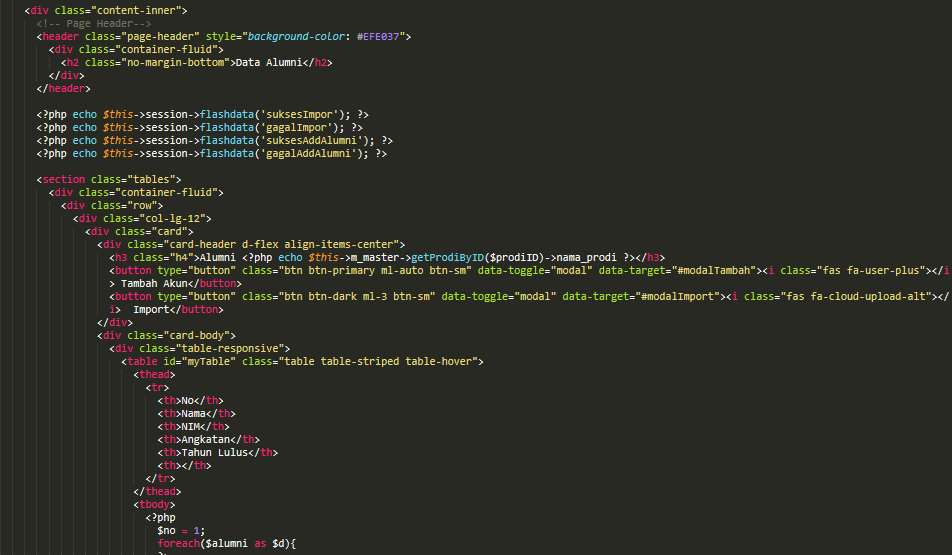
\includegraphics[width=14cm,height=7cm]{gambar/source_code/v_alumni}
	\caption{Struktur Pemrograman \textit{View}}
	\label{sc_vAlumni}
\end{figure}
